\documentclass[UTF8,zihao=-4]{ctexart}
\usepackage[a4paper,margin=2.5cm]{geometry}
\usepackage{amsmath, amssymb, amsthm}
\usepackage{bm}
\usepackage{hyperref}
\usepackage{graphicx}
\usepackage{caption}
\usepackage{listings}
\usepackage{xcolor}
\usepackage{float}
\usepackage{placeins}
\graphicspath{{figures/}}

% Code style
\lstdefinestyle{code}{
  basicstyle=\ttfamily\small,
  numbers=left,
  numberstyle=\tiny,
  numbersep=8pt,
  keywordstyle=\color{blue},
  commentstyle=\color{teal!70!black},
  stringstyle=\color{orange!70!black},
  showstringspaces=false,
  breaklines=true,
  frame=single,
  framerule=0.3pt,
  rulecolor=\color{black!15}
}
\lstset{style=code}

\title{深度强化学习:值函数、策略梯度与 AlphaGo}
\author{}
\date{\today}

\begin{document}
\maketitle
\tableofcontents
\FloatBarrier

\section{DQN、策略梯度、Actor-Critic}
深度强化学习将神经网络与强化学习目标结合,实现对复杂序列决策问题的端到端优化。图~\ref{fig:rl_overview_cn} 对比了值函数方法、策略梯度方法与 Actor-Critic 框架的核心流程。

\subsection{深度 Q 网络(DQN)}
DQN 近似离散动作空间下的最优动作价值函数 $Q^{\star}(s, a)$。贝尔曼最优方程为
\begin{equation}
  Q^{\star}(s, a) = \mathbb{E}_{s' \sim P(\cdot \mid s, a)} \left[ r(s, a) + \gamma \max_{a'} Q^{\star}(s', a') \right].
\end{equation}
DQN 使用神经网络 $Q_{\theta}(s, a)$ 拟合该函数,最小化时序差分(TD)损失:
\begin{equation}
  \mathcal{L}(\theta) = \mathbb{E}_{(s, a, r, s') \sim \mathcal{D}} \left[ \left( y - Q_{\theta}(s, a) \right)^2 \right], \quad y = r + \gamma \max_{a'} Q_{\theta^{-}}(s', a'),
\end{equation}
其中 $\theta^{-}$ 为周期性复制的目标网络参数,经验回放缓冲 $\mathcal{D}$ 用于打破样本相关性并提升数据效率。

\paragraph{稳定训练技巧}
\begin{itemize}
  \item \textbf{Double DQN:} 使用在线网络的 $\arg\max$ 选择动作,降低目标值的高估偏差。
  \item \textbf{Dueling 网络:} 将 $Q(s, a)$ 分解为状态价值 $V(s)$ 与优势函数 $A(s, a)$,提高不同动作值差异的表达力。
  \item \textbf{优先经验回放:} 根据 TD 误差大小调整采样概率,聚焦于训练困难样本。
\end{itemize}

\paragraph{伪代码}
\begin{lstlisting}[language=Python, caption={带目标网络与经验回放的 DQN 训练循环示例。}]
replay = ReplayBuffer(capacity=100_000)
q_net = QNetwork().to(device)
target_net = copy.deepcopy(q_net)
optimizer = torch.optim.Adam(q_net.parameters(), lr=1e-3)

for step in range(total_steps):
    action = epsilon_greedy(q_net, obs, epsilon_schedule(step))
    next_obs, reward, done, info = env.step(action)
    replay.add(obs, action, reward, next_obs, done)
    obs = next_obs if not done else env.reset()

    if step > warmup and step % train_freq == 0:
        batch = replay.sample(batch_size=64)
        target = batch.reward + gamma * target_net(batch.next_obs).max(dim=1).values * (1 - batch.done)
        q_values = q_net(batch.obs).gather(1, batch.action.unsqueeze(1)).squeeze(1)
        loss = F.mse_loss(q_values, target.detach())
        optimizer.zero_grad()
        loss.backward()
        clip_grad_norm_(q_net.parameters(), max_norm=10.0)
        optimizer.step()

    if step % target_update == 0:
        target_net.load_state_dict(q_net.state_dict())
\end{lstlisting}

\subsection{策略梯度方法}
策略梯度直接最大化期望回报 $J(\theta) = \mathbb{E}_{\tau \sim \pi_{\theta}} \left[\sum_{t=0}^{T} \gamma^{t} r_t\right]$。REINFORCE 梯度估计为
\begin{equation}
  \nabla_{\theta} J(\theta) = \mathbb{E}_{\pi_{\theta}} \left[ \sum_{t=0}^{T} \nabla_{\theta} \log \pi_{\theta}(a_t \mid s_t) \, G_t \right], \quad G_t = \sum_{k=t}^{T} \gamma^{k-t} r_k.
\end{equation}
为了降低方差,引入基线 $b(s_t)$ 后:
\begin{equation}
  \nabla_{\theta} J(\theta) = \mathbb{E}_{\pi_{\theta}} \left[ \sum_{t} \nabla_{\theta} \log \pi_{\theta}(a_t \mid s_t) \left( G_t - b(s_t) \right) \right].
\end{equation}
常见的基线包括学习得到的状态价值函数 $V_{\phi}(s)$,以及优势函数 $A_t = G_t - V_{\phi}(s_t)$。

\paragraph{信赖域与 PPO}
TRPO 通过约束新旧策略间的 KL 散度控制更新幅度。PPO 用易实现的截断代理目标替代:
\begin{align}
  L^{\text{CLIP}}(\theta) = \mathbb{E}\left[ \min\left( r_t(\theta) A_t, \operatorname{clip}(r_t(\theta), 1 - \epsilon, 1 + \epsilon) A_t \right) \right], \\
  r_t(\theta) = \frac{\pi_{\theta}(a_t \mid s_t)}{\pi_{\theta_{\text{old}}}(a_t \mid s_t)}.
\end{align}
广义优势估计(GAE)通过 $\lambda$-return 平滑优势,兼顾偏差与方差:
\begin{equation}
  A_t^{\text{GAE}} = \sum_{l=0}^{\infty} (\gamma \lambda)^l \delta_{t+l}, \quad \delta_t = r_t + \gamma V(s_{t+1}) - V(s_t).
\end{equation}

\subsection{Actor-Critic 框架}
Actor-Critic 同时学习策略(Actor)与价值(Critic)网络。Critic 估计 $V_{\phi}(s)$ 或 $Q_{\phi}(s, a)$ 用于降低方差。A2C/A3C 在同步/异步多线程环境下更新;Soft Actor-Critic (SAC) 在连续控制中引入熵正则:
\begin{equation}
  J_{\pi} = \mathbb{E}_{s_t \sim \mathcal{D}} \left[ \mathbb{E}_{a_t \sim \pi} \left[\alpha \log \pi(a_t \mid s_t) - Q_{\phi}(s_t, a_t)\right] \right],
\end{equation}
$\alpha$ 调节探索程度。DDPG、TD3 等确定性策略梯度方法针对连续动作设计。

\subsection{对比总结}
图~\ref{fig:rl_overview_cn} 总结了三类方法特点:
\begin{itemize}
  \item DQN:离散动作、离策略、依赖经验回放与目标网络。
  \item 策略梯度:在策略、适用于连续动作,但梯度方差较大。
  \item Actor-Critic:融合优点,实现稳定更新与连续控制。
\end{itemize}

\begin{figure}[H]
  \centering
  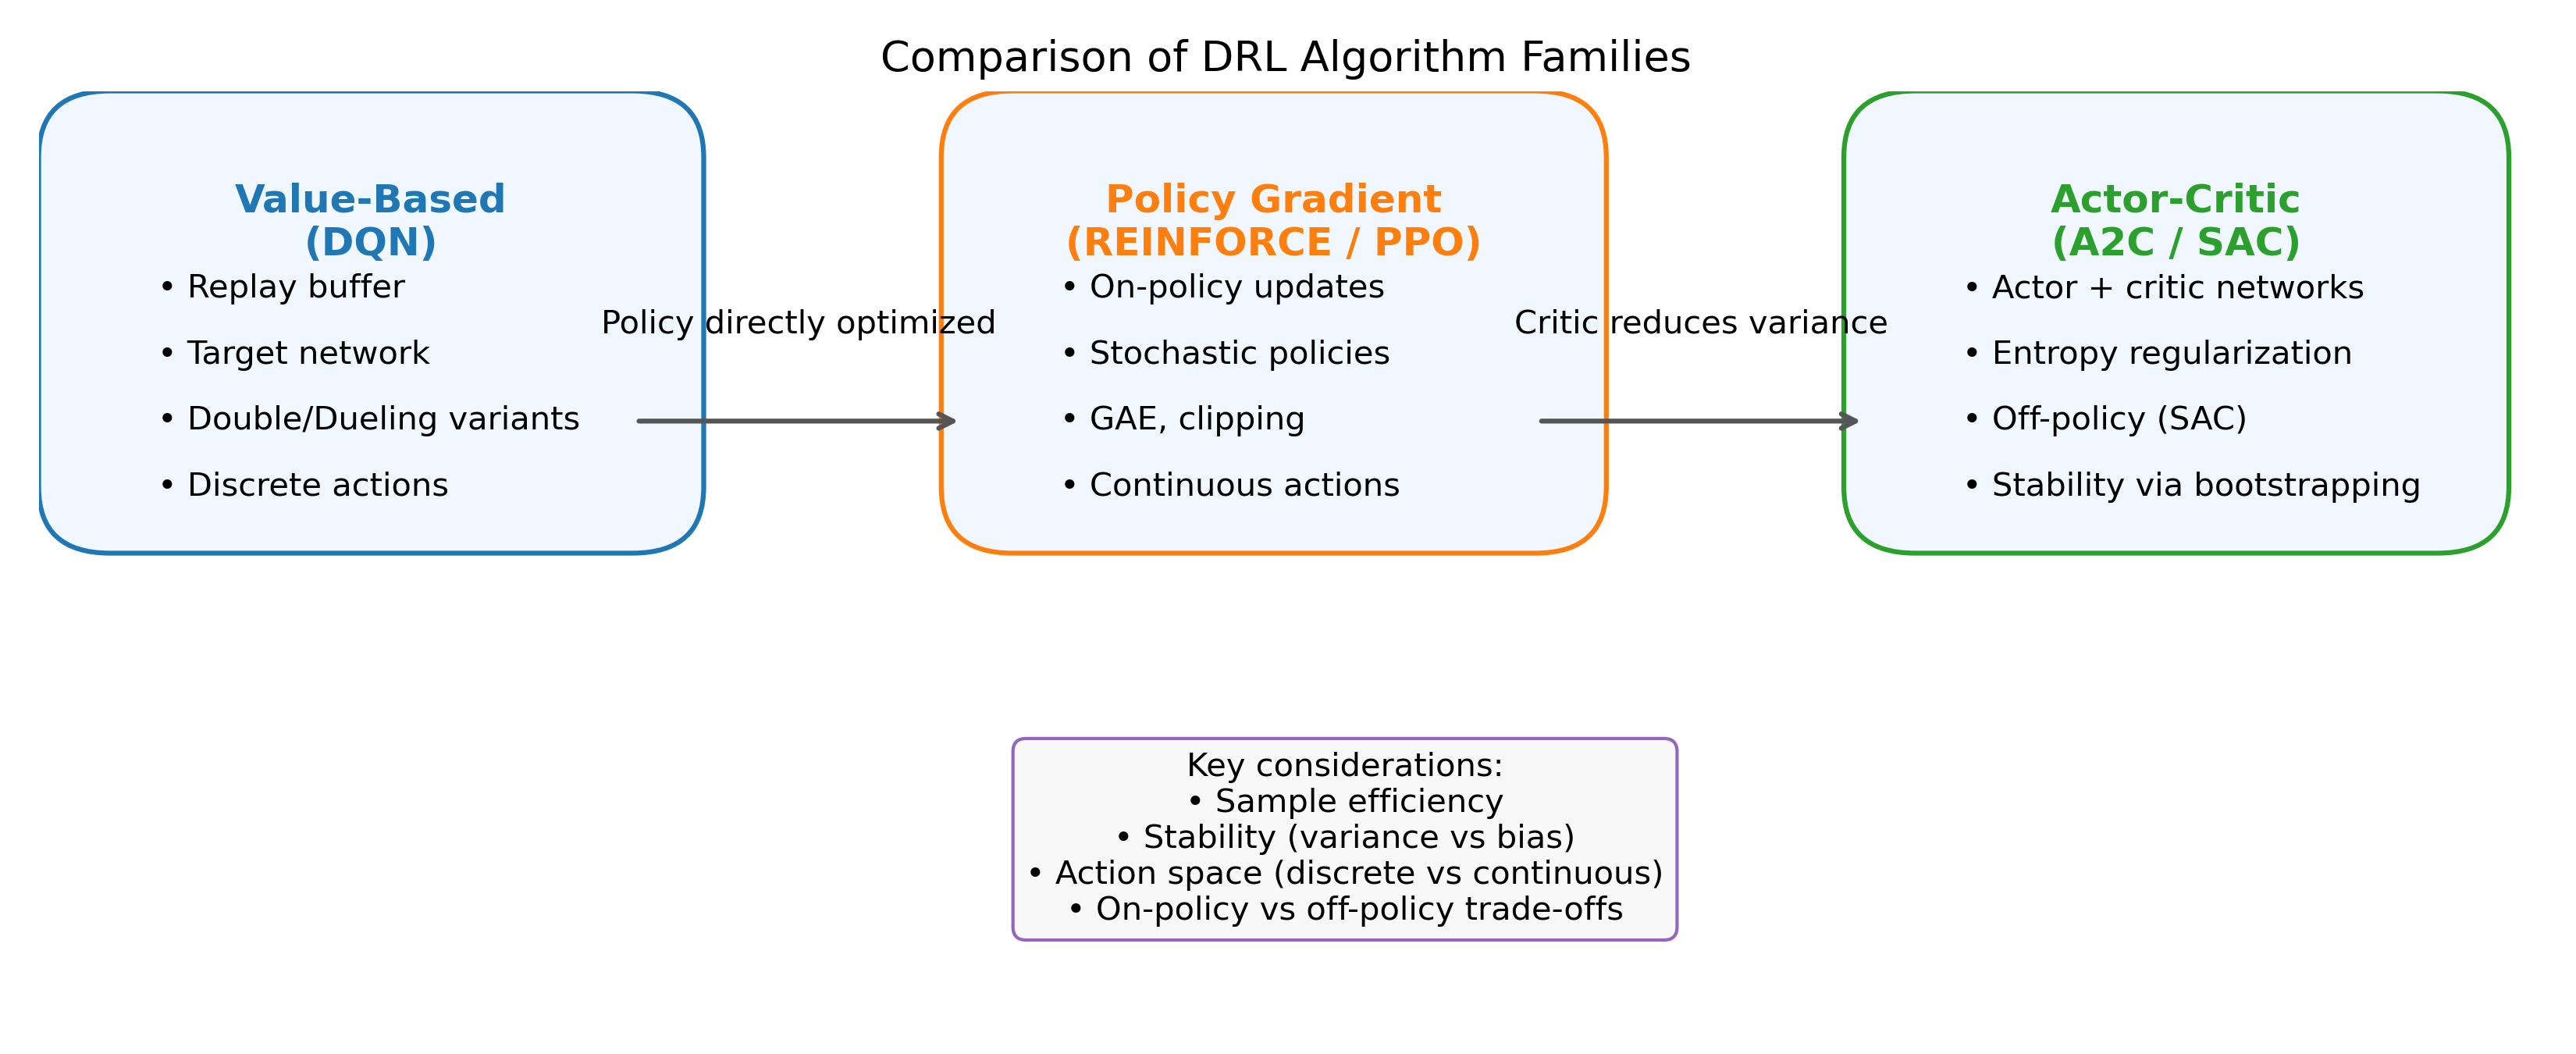
\includegraphics[width=0.9\textwidth]{rl_overview.png}
  \caption{DQN、策略梯度与 Actor-Critic 流水线对比。值函数方法依靠经验回放;策略梯度直接更新策略;Actor-Critic 融合两者优势。}
  \label{fig:rl_overview_cn}
\end{figure}
\FloatBarrier

\section{AlphaGo 案例}
AlphaGo 首次将深度神经网络与蒙特卡罗树搜索(MCTS)结合,实现围棋超越人类顶尖水平。图~\ref{fig:alphago_pipeline_cn} 展示了监督学习、强化学习与树搜索的组合流程。

\subsection{策略网络训练}
监督策略网络 $p_{\theta}(a \mid s)$ 在职业棋谱上通过交叉熵训练:
\begin{equation}
  \mathcal{L}_{\text{SL}}(\theta) = -\mathbb{E}_{(s, a) \sim \mathcal{D}_{\text{human}}} [\log p_{\theta}(a \mid s)].
\end{equation}
随后基于自对弈进行策略梯度优化,最大化胜率 $\rho(\theta)$:
\begin{equation}
  \nabla_{\theta} \rho(\theta) = \mathbb{E}_{\tau \sim p_{\theta}} \left[ \left( z - b \right) \sum_{t} \nabla_{\theta} \log p_{\theta}(a_t \mid s_t) \right],
\end{equation}
其中 $z \in \{-1, +1\}$ 为对局结果,$b$ 为基线减少方差。

\subsection{价值网络与快速模拟}
价值网络 $v_{\phi}(s)$ 预测当前局面的胜率,使用自对弈样本与蒙特卡罗结果训练:
\begin{equation}
  \mathcal{L}_{\text{value}}(\phi) = \mathbb{E}_{s \sim \mathcal{D}_{\text{self-play}}} \left[ \left( v_{\phi}(s) - z \right)^2 \right].
\end{equation}
搜索过程中还使用轻量快速走子策略进行随机模拟,以提升评估多样性。

\subsection{MCTS 融合}
AlphaGo 在树搜索中采用改进的上置信界(PUCT)选择:
\begin{equation}
  a_t = \arg\max_{a} \left( Q(s_t, a) + c_{\mathrm{puct}} \, P(s_t, a) \frac{\sqrt{ \sum_b N(s_t, b) }}{1 + N(s_t, a)} \right),
\end{equation}
其中 $Q$ 为平均回报,$P$ 为策略网络先验,$N$ 为访问次数。策略网络用于引导扩展节点,价值网络提供评估,大幅压缩搜索空间。

\subsection{AlphaGo Zero 与 AlphaZero}
AlphaGo Zero 取消监督阶段,通过纯自对弈学习,将策略和值合并为一个残差网络输出 $(p, v)$。策略目标为 MCTS 访问频率 $\pi$,损失函数为
\begin{equation}
  \mathcal{L}(\theta) = (z - v_{\theta}(s))^2 - \pi^{\top} \log p_{\theta}(s) + \lambda \|\theta\|^2.
\end{equation}
AlphaZero 将该框架推广至国际象棋、将棋,证明树搜索 + 自对弈的通用性。

\subsection{工程启示}
\begin{itemize}
  \item \textbf{硬件集群:} AlphaGo 结合 GPU 评估网络与分布式 CPU 树搜索,高效调度计算资源。
  \item \textbf{训练效率:} 自对弈数据进入回放缓冲,确保训练样本多样且可重复使用;批量化树搜索调用提升硬件利用率。
  \item \textbf{评估体系:} 使用 Elo 评分对比历史版本,进行模块消融试验,并与顶级棋手对战检验实力。
\end{itemize}

\begin{figure}[H]
  \centering
  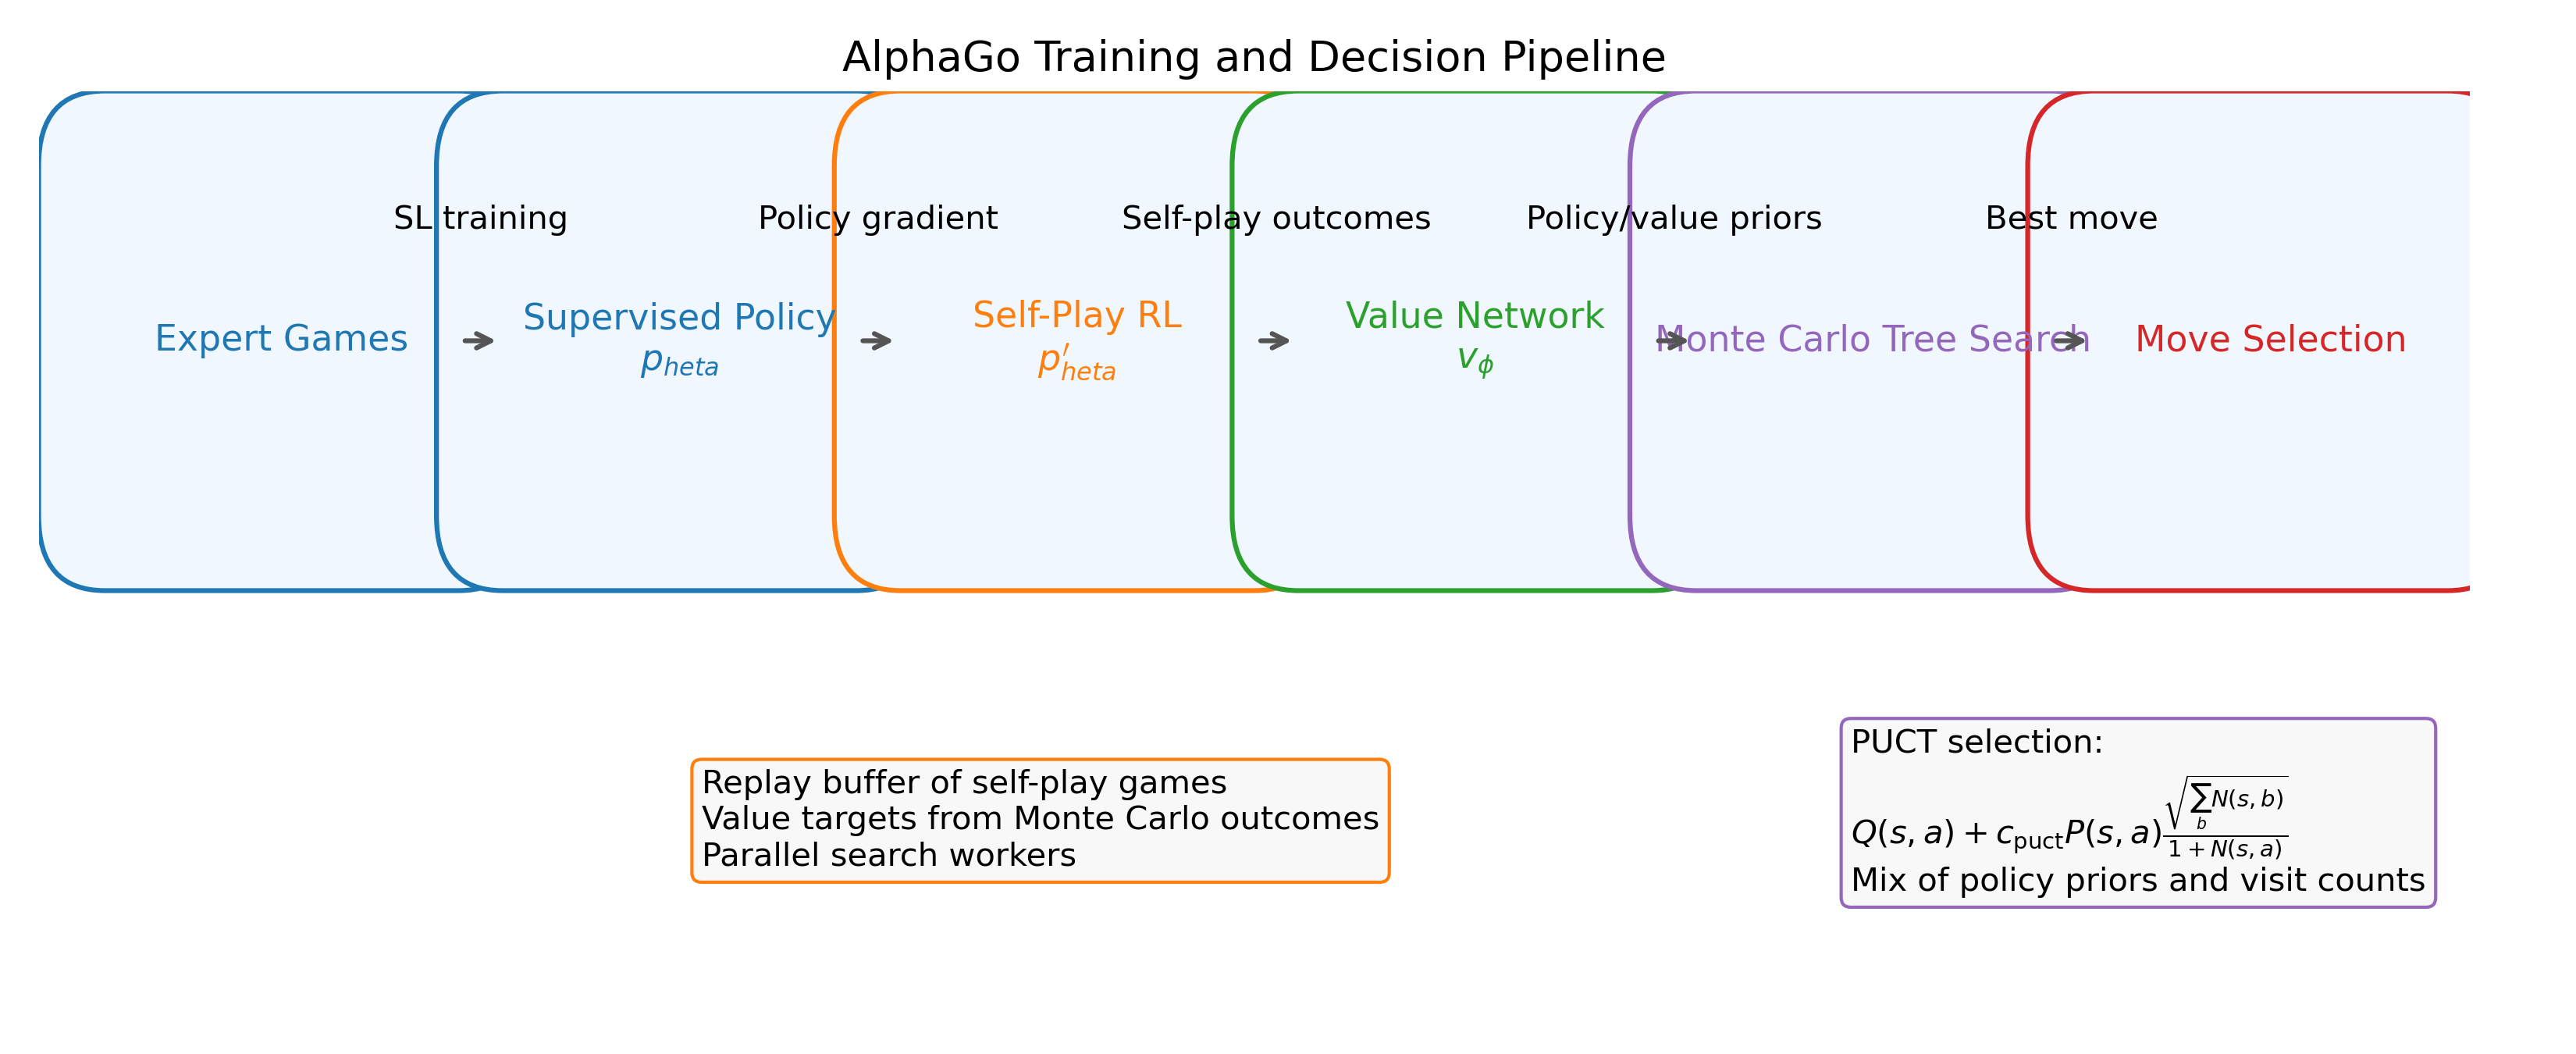
\includegraphics[width=0.9\textwidth]{alphago_pipeline.png}
  \caption{AlphaGo 训练与推理流程:监督策略初始化、自对弈强化学习、价值网络训练与 MCTS 决策。}
  \label{fig:alphago_pipeline_cn}
\end{figure}
\FloatBarrier

\section*{延伸阅读}
\begin{itemize}
  \item Volodymyr Mnih 等:《Playing Atari with Deep Reinforcement Learning》,2013。
  \item John Schulman 等:《Proximal Policy Optimization Algorithms》,2017。
  \item Tuomas Haarnoja 等:《Soft Actor-Critic Algorithms and Applications》,2018。
  \item Silver 等:《Mastering the game of Go with deep neural networks and tree search》,Nature 2016。
  \item Silver 等:《Mastering Chess and Shogi by Self-Play with a General Reinforcement Learning Algorithm》,2017。
\end{itemize}

\end{document}
